\documentclass[11pt]{article}
\usepackage[margin=0.68in]{geometry}

\usepackage{amsmath,amssymb}
\usepackage{booktabs}
\usepackage{graphicx}
\usepackage{xcolor}
\usepackage{hyperref}
\usepackage{enumitem}
\usepackage{microtype}
\usepackage{titlesec}
\usepackage{float}

\hypersetup{colorlinks=true,linkcolor=black,urlcolor=blue!50!black}
\titleformat{\section}{\large\bfseries}{\thesection}{0.55em}{}
\setlength{\parskip}{0.28em}
\setlength{\parindent}{0pt}
\setlist[itemize]{leftmargin=1.15em,itemsep=0.1em,topsep=0.15em}
\setlist[enumerate]{leftmargin=1.15em,itemsep=0.1em,topsep=0.15em}
\floatplacement{figure}{H}
\floatplacement{table}{H}

\title{\textbf{Perry--Beurling Spectral Sieve:\\
Status Note on Diagnostic Lemmas and\\
Grand Arithmetic Campaign}}
\author{Nicholas Perry\\[0.2em]
\textit{Private research note --- not a proof of RH}\\[0.15em]
\normalsize\texttt{luckyseoul/perry-beurling-spectral-sieve}}
\date{26 July 2026}

\begin{document}
\maketitle
\vspace{-1.4em}

\begin{abstract}
\noindent
We summarize the reconstructed Perry--Beurling Spectral Sieve (PBSS): a projection
diagnostic for density residuals on log-windows, with model theorems A$_0$/B$_0$ proved
as lemmas M1--M4, and a grand numerical campaign of the arithmetic Chebyshev residual
through \(x_{\max}=10^{10}\). The instrument behaves as designed on critical-line and
defect controls. The arithmetic residual soft-plateaus at \(R_d\approx 0.15\)--\(0.19\)
and does \emph{not} exhibit A$_0$-style collapse. Full Theorems A and B, and the
Riemann Hypothesis, remain open. This note is a status brief with diagrams, not a
submission claiming RH.
\end{abstract}

\section{Setup}
Fix a logarithmic window length \(T>0\) and set \(x=e^{uT}\) for \(u\in[0,1]\).
Let \(\{\varphi_k\}_{k\ge 0}\) be the shifted Legendre orthonormal system on
\(L^2([0,1],du)\):
\[
\varphi_k(u)=\sqrt{2k+1}\,L_k(2u-1),\qquad
V_d=\operatorname{span}\{\varphi_0,\ldots,\varphi_d\},\quad P_d=\text{proj.\ onto }V_d.
\]
For a residual \(q\in L^2([0,1])\) define the energy ratio
\[
R_d(q)
=\frac{\|P_d q\|_{L^2}^2}{\|q\|_{L^2}^2}
=\frac{\sum_{k=0}^{d}|\langle q,\varphi_k\rangle|^2}{\|q\|^2}\in[0,1],
\qquad
S_d(q;T)=T^{2(d+1)}R_d(q).
\]
Low \(R_d\): high-frequency content (RH-like for pure critical-line modes).
High \(R_d\): persistent low-degree mass (defect).

\begin{figure}[H]
\centering
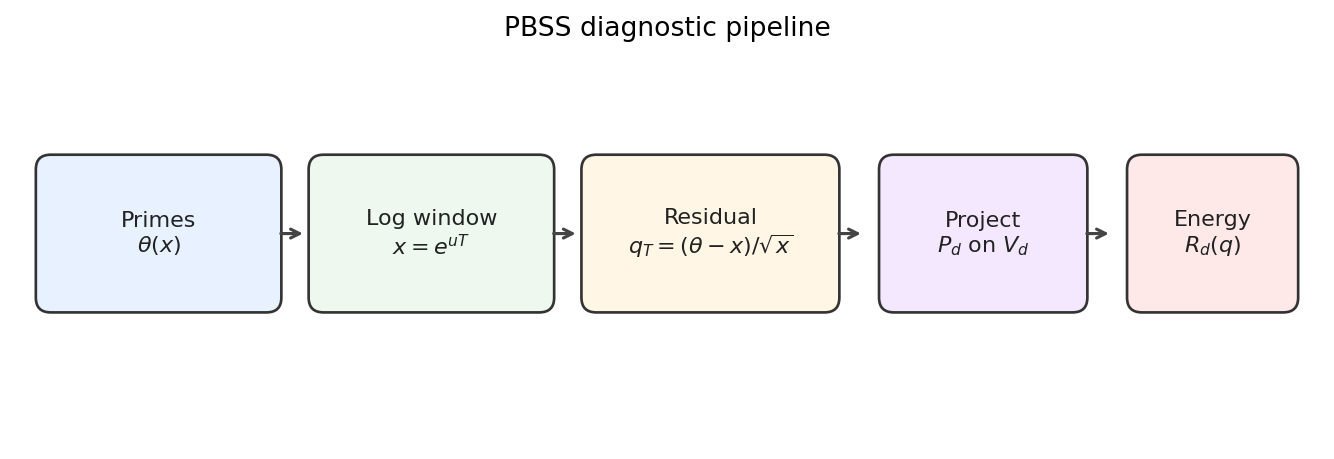
\includegraphics[width=0.94\textwidth]{figures/pipeline.png}

\caption{Diagnostic pipeline: Chebyshev residual on a log-window, projected onto
low-degree Legendre modes; report \(R_d\).}
\end{figure}

\paragraph{Model residuals.}
Critical-line (CL) mode \(q_T^{\mathrm{cl}}(u)=\sin(tTu)\); off-critical
\(e^{T(\sigma-1/2)u}\sin(tTu)\); orthogonal defect
\(q=\sqrt{1-\varepsilon^2}\,f+\varepsilon\,\varphi_j\) with \(f\perp V_d\), \(\|f\|_2=1\).

\paragraph{Arithmetic residual (shipped probe).}
With \(\theta(x)=\sum_{p\le x}\log p\),
\[
q_T(u)=\operatorname{detrend}\!\Bigl(\frac{\theta(e^{uT})-e^{uT}}{\sqrt{e^{uT}}}\Bigr)
\quad\text{(default detrend: degree one).}
\]

\section{Proved diagnostic lemmas (A$_0$/B$_0$)}
\begin{center}
\small
\begin{tabular}{@{}cl@{}}
\toprule
\textbf{Lemma} & \textbf{Statement} \\
\midrule
M1 & \(R_d(\varphi_m)=1_{m\le d}\) \\
M2 & Orthogonal defect \(\Rightarrow R_d(q)=\varepsilon^2\) \\
M3 & CL pure mode \(R_d(\sin(tTu))=O_d(T^{-2})\) \textbf{(A$_0$)} \\
M4 & Fixed \(\varepsilon>0\Rightarrow R_d\not\to 0\) (blocks vanishing) \\
\bottomrule
\end{tabular}
\end{center}

M1--M4 are continuous \(L^2\) arguments (\texttt{src/pbss/lemmas.py}) with discrete
verification in \texttt{tests/}. They prove the \emph{model} theorems:
\begin{itemize}
\item \textbf{A$_0$ (proved):} critical-line pure mode has \(R_d\to 0\) as \(T\to\infty\).
\item \textbf{B$_0$ (proved):} a uniform low-degree defect keeps \(R_d=\varepsilon^2\not\to 0\).
\end{itemize}
Vanishing of \(R_d\) is \emph{necessary} for the absence of a persistent polynomial defect.
It is \emph{not} a proof that arithmetic primes are free of such structure, nor a proof of RH.

\begin{figure}[H]
\centering
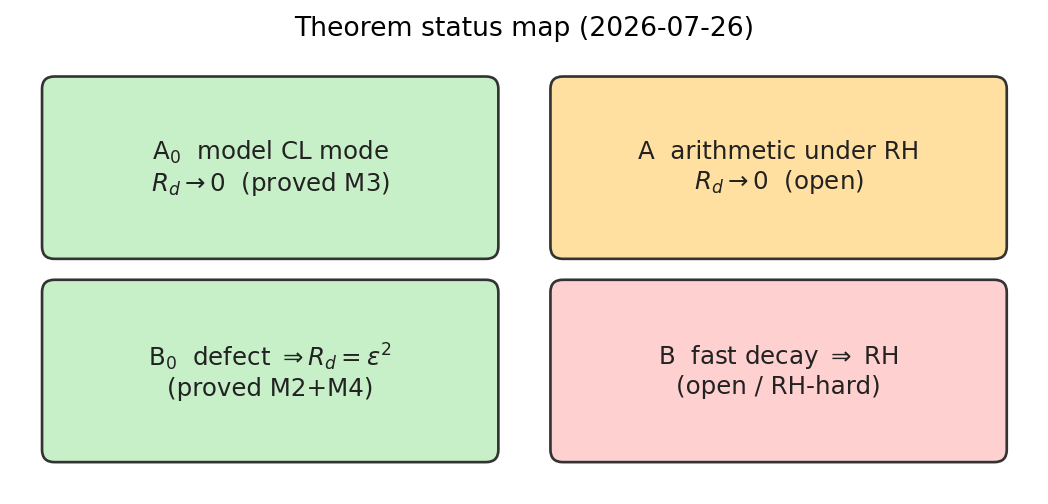
\includegraphics[width=0.78\textwidth]{figures/status_map.png}

\caption{Status map. Green: proved model results. Amber/red: full A/B open.}
\end{figure}

\section{Theorems A and B (open beyond models)}
\paragraph{Full Theorem A (conditional on RH; open).}
Under RH, for the arithmetic residual \(q_T\) (or an equivalent explicit-formula residual),
\(R_d(q_T)\to 0\) as \(T\to\infty\). Outline: RH \(\Rightarrow\) superposition of CL modes;
each contributes \(O(T^{-2})\) by M3; controlling the sum over zeros is analytic number theory
not completed here.

\paragraph{Full Theorem B (open; RH-hard).}
If \(R_d(q_T)\) decays sufficiently fast, then \(\zeta\) has no zero off the critical line.
The implication is essentially as hard as RH; not proved in this repository.

\section{Grand campaign numerics}
Runner: \texttt{experiments/run\_grand\_campaign.py}.
Scale: \(x_{\max}=10^{10}\) (455\,052\,511 primes, segmented sieve + on-disk checkpoint);
14 windows in \(T\); ablations \(d\in\{2,4,6,8\}\),
detrend \(\in\{\mathrm{none},\mathrm{deg0},\mathrm{deg1}\}\);
controls CL / off-critical \(\sigma{=}0.75\) / defect \(\varepsilon{=}0.5\);
\textbf{20\,000} MC spectral-defect trials per \(T\) (280\,000 total);
wall \(\sim 1\) hour multi-core; resume-capable state JSON.

\begin{table}[H]
\centering
\caption{Focus cut (\(d=4\), deg1) and controls at large \(T\).}
\small
\begin{tabular}{@{}rrrrrr@{}}
\toprule
\(T\) & \(x_{\max}\) & \(R_4\) arith & \(R_4\) CL & \(R_4\) defect & MC mean \\
\midrule
10 & \(2{\times}10^{4}\) & 0.144 & \({\sim}6{\times}10^{-3}\) & 0.250 & 0.793 \\
16 & \(9{\times}10^{6}\) & 0.193 & \({\sim}2{\times}10^{-3}\) & 0.250 & 0.793 \\
23 & \(1{\times}10^{10}\) & \textbf{0.155} & \({\sim}5{\times}10^{-4}\) & 0.250 & 0.795 \\
\bottomrule
\end{tabular}
\end{table}

\begin{figure}[H]
\centering
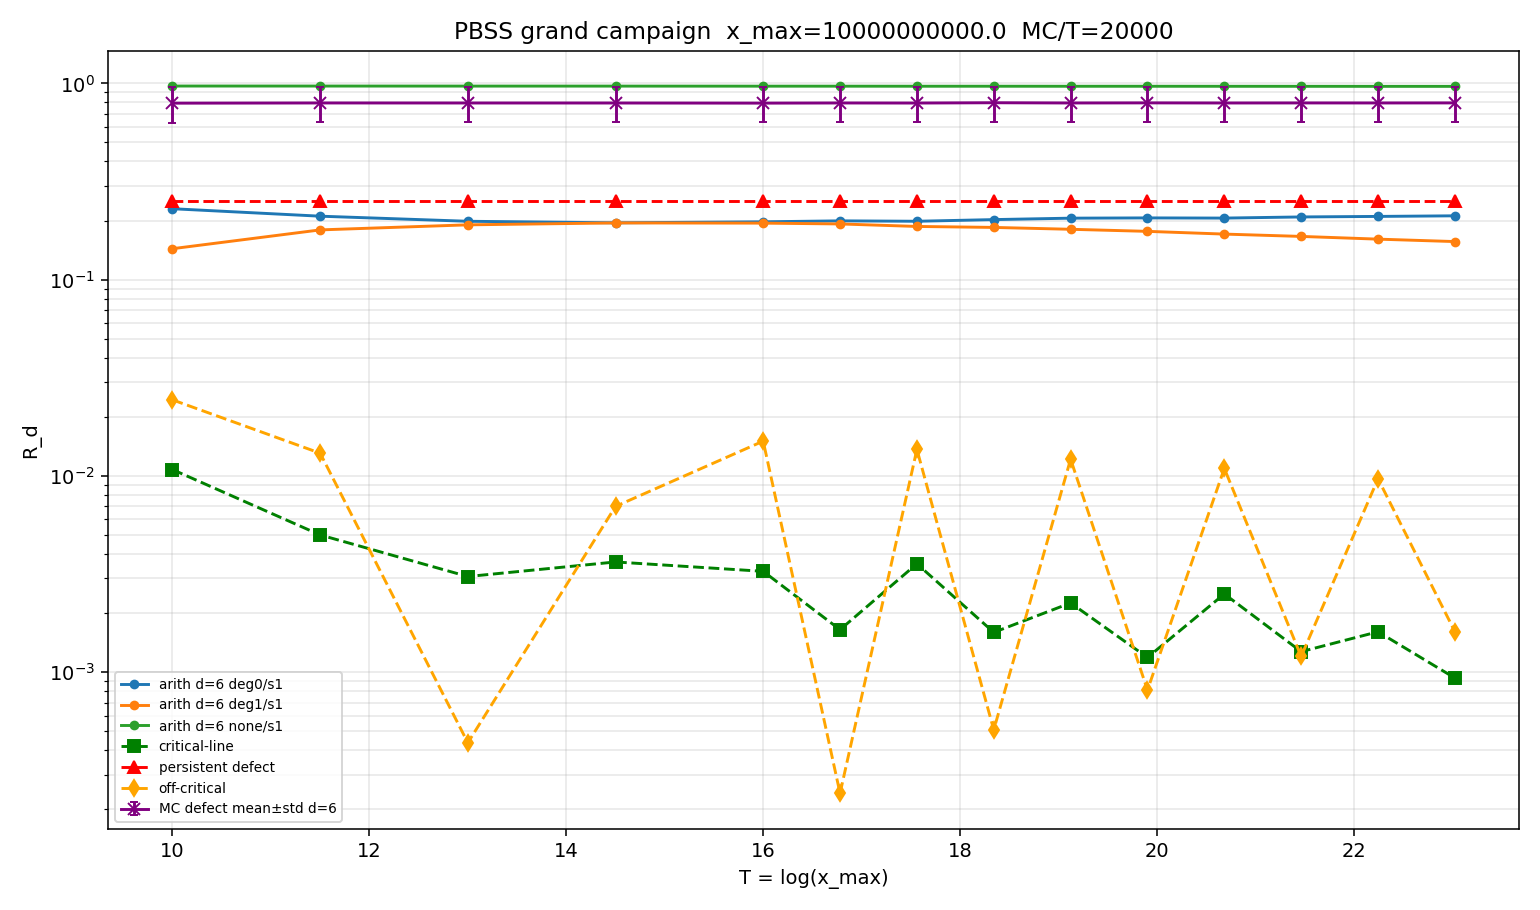
\includegraphics[width=0.86\textwidth]{figures/grand_Rd_vs_T.png}

\caption{Grand campaign: arithmetic ablations, CL/defect/off-critical controls, MC defect
mean \(\pm\) std. Arithmetic tracks stay \(O(10^{-1})\); CL decays; defects stay high.}
\end{figure}

\begin{figure}[H]
\centering
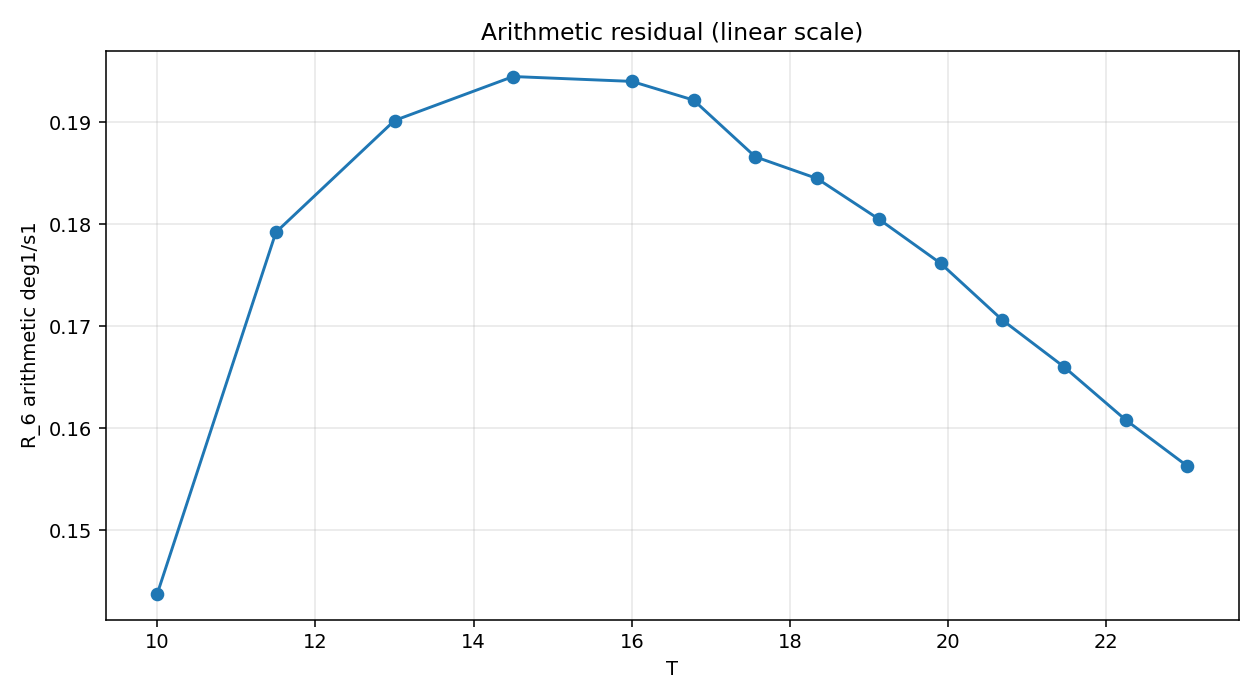
\includegraphics[width=0.72\textwidth]{figures/grand_arith_focus_linear.png}

\caption{Arithmetic focus on a linear \(R_d\) scale: soft plateau \(\sim 0.15\)--\(0.19\)
through \(T\approx 23\) (\(x_{\max}=10^{10}\)).}
\end{figure}

\paragraph{Reading.}
\begin{enumerate}
\item The diagnostic separates pure CL modes from planted defects as A$_0$/B$_0$ predict.
\item Arithmetic \(q_T=(\theta-x)/\sqrt{x}\) (detrended) does \textbf{not} collapse like A$_0$
through ten billion; it soft-plateaus.
\item This does \textbf{not} prove or disprove RH. The current arithmetic probe is not yet
the object for which full Theorem A is numerically visible.
\end{enumerate}

\section{Done vs open; next step}
\begin{center}
\small
\begin{tabular}{@{}p{0.46\textwidth}p{0.46\textwidth}@{}}
\toprule
\textbf{Done} & \textbf{Open} \\
\midrule
Lemmas M1--M4; A$_0$/B$_0$ & Full Theorem A (arithmetic under RH) \\
Sieve + checkpoint to \(10^{10}\) & Full Theorem B \\
Grand multi-\(T\) ablations, MC & Explicit-formula residual / zero-peeling \\
Optional CuPy (NumPy fallback) & Finite-mode sum lemma; stronger whitening \\
Tests green; docs locked & Legacy \(P\approx 3.92\) normalization \\
\bottomrule
\end{tabular}
\end{center}

\paragraph{Highest-leverage next step.}
Build an \emph{explicit-formula residual}: subtract truncated zero sums / secondary main terms,
then re-project. Couple with a proved finite-superposition form of M3. Larger \(x\) alone
mostly reconfirms the plateau; the A-gap is the missing bridge from arithmetic \(q_T\) to
CL mode sums.

\section{Explicit non-claim}
\begin{quote}
\itshape
This repository and this note do not contain an unconditional proof of the Riemann Hypothesis.
Proved results are about the diagnostic (A$_0$/B$_0$). Full A/B and RH remain open.
\end{quote}
\noindent
Artifacts: \texttt{docs/STATUS.md}, \texttt{THEOREMS\_AB.md}, \texttt{PROOFS\_LEMMAS.md},
\texttt{results/grand\_campaign/}. Private research; not for public distribution without permission.

\end{document}
